\section{High modulus polyethylene}
High modulus polyethylene (HMPE) or ultra-high-molecular-weight polyethylene (UHMWPE) is so called because it consists of very long chains of polyethylene. Having a longer chain length than other forms of polyethylene, HMPE has more interaction between different chains, and thus has a higher stiffness, despite the low strength of the individual van der Waals bonds.

\subsection{Production}
Initially, long polyethylene fibres (``macrofibrillar crystals'') were produced from a solution of linear polyethylene (figure \ref{fig:pe}), which is mostly linear with only short branches, in p-xylene (figure \ref{fig:p-xylene}). A long crystal was grown from the side of a rotating cylinder containing the solution (figure \ref{fig:grow_pe}). This produced fibres which reduced in diameter as they grew, and so were not particularly useful \pcite{zwijnenburg_longitudinal_1976}.

\newcommand\setpolymerdelim[2]{\def\delimleft{#1}\def\delimright{#2}}
\def\makebraces[#1,#2]#3#4#5{%
\edef\delimhalfdim{\the\dimexpr(#1+#2)/2}%
\edef\delimvshift{\the\dimexpr(#1-#2)/2}%
\chemmove{%
\node[at=(#4),yshift=(\delimvshift)]
{$\left\delimleft\vrule height\delimhalfdim depth\delimhalfdim
width0pt\right.$};%
\node[at=(#5),yshift=(\delimvshift)]
{$\left.\vrule height\delimhalfdim depth\delimhalfdim
width0pt\right\delimright_{\rlap{$\scriptstyle#3$}}$};}}
\setpolymerdelim()
\begin{figure}
\centering
\chemfig{\vphantom{CH_2}-[@{op,.75}]CH_2-CH_2-[@{cl,0.25}]}
\makebraces[5pt,5pt]{\!\!n}{op}{cl}
\caption{Polyethylene's repeating unit}
\label{fig:pe}
\end{figure}

\begin{figure}
\centering
\chemfig{H_3C-*6(-=-(-CH_3)=-=)}
\caption{p-xylene molecule}
\label{fig:p-xylene}
\end{figure}

\begin{figure}
\centering
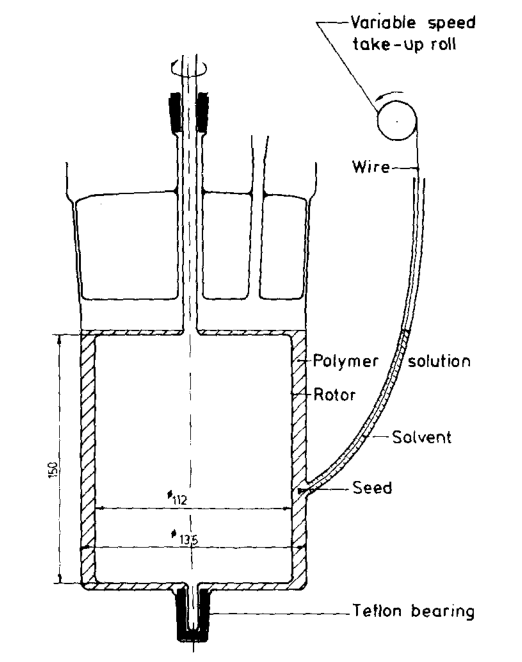
\includegraphics[width=0.8\columnwidth]{images/growing_polyethylene}
\caption{Growing polyethylene fibres using a Couette instrument \pcite{zwijnenburg_longitudinal_1976}}
\label{fig:grow_pe}
\end{figure}

A more easily commercialised method of production is the spinning and drawing of polyethylene filaments. The solution containing polyethylene is extruded through small nozzles in a spinneret \pcite{polymer_spinning}, producing a polyethylene fibre, and this goes through a cooling bath and then an oven at \SI{120}{\celsius}---below the melting point of the polymer.

While in the oven, in the method of \cite{smith_ultra-high-strength_1980} the fibres are stretched at a strain rate of around \SI{1}{\per\second}, which aligns the polyethylene chains. Smith and Lemstra explain that the fibre is stretched after being cooled because it reduces the relaxation effect---in the liquid state macromolecules exhibit a ``relatively rapid relaxation''. The oven drawing has the added benefit of evaporating all detectable quantities of the solvent from the fibres, leaving only polyethylene.

\subsection{Properties}
This method produces polyethylene fibres with a tensile strength and modulus dependent on the draw ratio. The draw ratio is the ratio of the cross-sectional area of the un-drawn fibres to that of the drawn ones.

As you can see from figure \ref{fig:pe_fibre_ss}, as the polymer is drawn out more, the ultimate tensile strength increases, up to \SI{3.04}{\giga\pascal} at a ratio of $31.7$. This shows that the increased crystallinity caused by drawing the fibres does have a positive effect on the tensile strength.

The modulus of Smith and Lemstra's most highly drawn polyethylene is \SI{90.2}{\giga\pascal}, around half that of steel. The fibre makes up for its lower stiffness with a much higher tensile strength than steel.

\begin{figure}
\centering
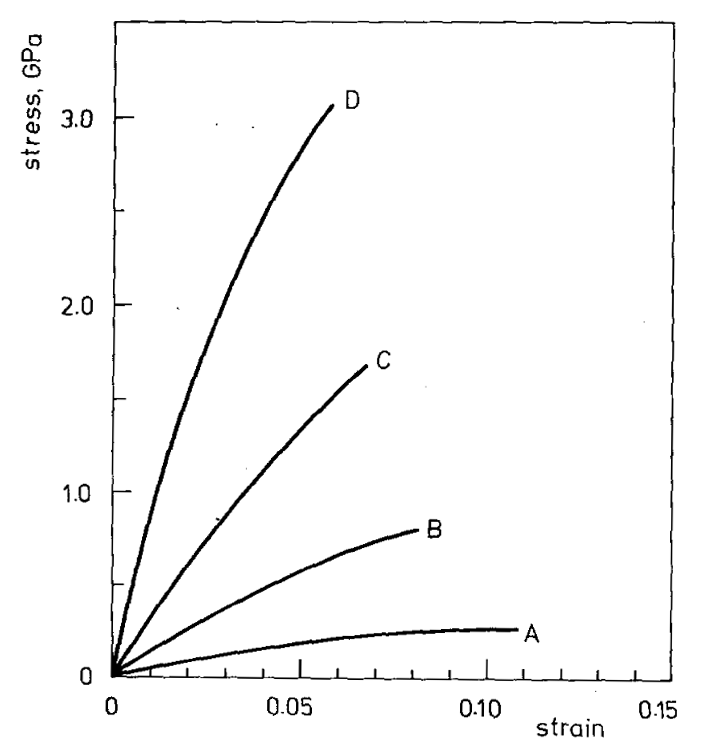
\includegraphics[width=0.8\columnwidth]{images/pe_stress_strain}
\caption{Stress-strain curves of polyethylene fibres. Draw ratios: A 2.8; B 8.4; C 15.7; D 31.7 \pcite{smith_ultra-high-strength_1980}}
\label{fig:pe_fibre_ss}
\end{figure}

\subsubsection{Effects of crosslinking}
Another application for which UHMWPE is used is  human joint replacement, in which the polymer acts as a synthetic cartilage. In the lower part of the knee joint, the polymer "undergoes cyclic stresses as high as \SIrange{10}{15}{\mega\pascal} in tension and \SIrange{30}{40}{\mega\pascal} in compression" \pcite{simis_combined_2006}. Simis et.\ al.\ explore the effects of crosslinking on the microstructural and mechanical properties of UHMWPE.

The extra crosslinks were created by subjecting samples of the polymer to ionising radiation. The source used was a \SI{5}{\kilo\gray} gamma ray source. The samples were then held above their melting temperature at \SI{170}{\celsius} for \SI{4}{\hour} "to complete the crosslinking and annihilate free radicals" \pcite{simis_combined_2006}. High pressure variants were created by subjecting the polyethylene to pressures of \SI{500}{\mega\pascal} shortly before cooling.

All specimens had a layered appearance in their microstructure, but that of the irradiated specimens had a much smaller lamellae thickness. This was especially apparent in the high pressure variant, where the thickness was \SI{50.6}{\nano\metre} compared to the non-irradiated specimen's \SI{131.2}{\nano\metre}.

The effect this has on the properties is unexpected. The tensile modulus is decreased in the low-pressure variants, and there is only a statistically insignificant increase in the high pressure variant. What this means is that the increased cross-linking does not have a positive effect on the modulus.

The ultimate tensile strength, however, is (at least for the high pressure samples) increased from \SI{78.8}{\mega\pascal} to \SI{167.8}{\mega\pascal}. The low-pressure variants show an equally significant decrease in tensile strength.

\cite{muratoglu_unified_1999} note that while a number of mechanical properties are decreased by the increased crosslinking, the wear resistance does increase, which was the aim of the original experiments by \cite{simis_combined_2006}

What this means is that while the radiation-induced crosslinking has produced an interesting effect on the microstructure of the polymer, it has not had an effect which would be useful for hammock suspension.

\subsection{How the properties are useful}